\documentclass[sigconf]{acmart}
\AtBeginDocument{%
  \providecommand\BibTeX{{%
    Bib\TeX}}}
\usepackage{siunitx}
\usepackage{bm}
\settopmatter{printacmref=false}
\setcopyright{none}

%% Rights management information.  This information is sent to you
%% when you complete the rights form.  These commands have SAMPLE
%% values in them; it is your responsibility as an author to replace
%% the commands and values with those provided to you when you
%% complete the rights form.
\setcopyright{acmlicensed}
\copyrightyear{2018}
\acmYear{2025}
\acmDOI{https://doi.org/10.1145/3576781.3608719}
%% These commands are for a PROCEEDINGS abstract or paper.
\acmConference[NANOCOM '25]{Proceedings of the 10th ACM International Conference on Nanoscale Computing and Communication}{June 03--05,
  2025}{Coventry, United Kingdom}
%%
%%  Uncomment \acmBooktitle if the title of the proceedings is different
%%  from ``Proceedings of ...''!
%%
%%\acmBooktitle{Woodstock '18: ACM Symposium on Neural Gaze Detection,
%%  June 03--05, 2018, Woodstock, NY}
\acmISBN{978-8-4007-0034-7/23/09...\$15.00}           
%%%%%%%%%%%%%%%%%%%%%%%%%%%%%%%%%%%%%%%%%%%%%%%%%%%%%%%%%%%%%%%%%%%%%%%%%%%%%%%%%%%%%%%%%%%%%%%%%%%%%%%%%%%%%%%%%%%%%%%%%%%%%%%%%%%%%
\begin{document}

\title{In Silico Model for Tumor Diagnosis Based on Bloodstream Penetrating Extracellular Vesicles}
\author{Robin Brendel}
\email{robin.brendel@student.uni-luebeck.de}
\affiliation{%
  \institution{University of Lübeck}
  \state{Schleswig-Holstein}
  \country{Germany}
}

\begin{abstract}
\textit{Extracellular vesicles (EVs)} have drawn a lot of scientific attention in the last ten years as natural drug carriers and disease biomarkers, particularly for cancer. Although a few studies have monitored tumor-derived EVs in the bloodstream or extracellular spaces, none have fully modeled their concurrent passage through surrounding tissues, blood vessels, and tumor microenvironments. We created an in silico computer model that replicates the entire procedure. Our model includes EV release from cancer cells, circulation through arterial-capillary-venous networks, transport across tissue, and eventual bloodstream entry. Based on the speed at which tumor EVs enter the bloodstream, we suggest a novel diagnostic approach for sub-millimeter tumors by examining simulation results. Our results highlight the method's sensitivity to tumor size and its potential for non-invasive cancer detection. 
\end{abstract}

\begin{CCSXML}
<ccs2012>
 <concept>
  <concept_id>10010147.10010257.10010291</concept_id>
  <concept_desc>Applied computing~Computational biology~Systems biology</concept_desc>
  <concept_significance>500</concept_significance>
 </concept>
</ccs2012>
\end{CCSXML}

\ccsdesc[500]{Applied computing~Systems biology}

\keywords{In Silico, Extracellular Vesicles, COMSOL, Tumor, Diagnosis, Cancer, Biomarkers}

\maketitle

\section{Introduction}
\label{sec: introduction}
EVs are tiny lipid-bound particles, 30 nm to \SI{5}{\micro\meter} in size, released by cells into their surroundings \cite{Doyle_2019}. Their lipid walls protect contents from enzymes and help cross biological barriers \cite{Arjmandi_2021}. Combining durability, natural targeting, and cargo-specificity\cite{Piffoux_2018}, EVs offer exciting potential as diagnostic biomarkers and natural drug delivery vehicles, particularly for cancer \cite{Doyle_2019}. Since EVs do not move locally, they can enter the bloodstream and travel systemically with the blood flow. This enables non-invasive diagnostics, prompting mathematical models of EV blood propagation \cite{Ferguson_2020}. Understanding this tissue-blood journey is crucial for improving diagnostics and drug delivery. 

For an overview of these mechanisms the following paper is given \cite{Sykov__2008}. Beyond expensive invasive studies in vivo or limited experiments in vitro, computer models provide cost-effective in silico alternatives that can show complex biological processes while reducing experiments in the lab. 

\section{System Model}
\label{subsec: sys-model}
Figure 1 shows our realistic biological scenario with the following distinct zones: the artery functioning as blood inlet, vein as blood outlet, capillary network ($\Omega_{\text{c}}$), tumor area ($\Omega_{\text{t}}$), and healthy tissue ($\Omega_{\text{h}}$). 

Since tumors need oxygen and nutrients, capillaries infiltrate cancerous regions. Tumor-generated EVs can either penetrate capillary walls into blood or migrate into healthy tissue. The bloodstream entry rate depends on vessel wall permeability which is modeled by:
\begin{displaymath}
  k_{\mathrm{p}}=\frac{D_{\mathrm{w}}}{d_{\mathrm{w}}},
\end{displaymath}

where $D_{\mathrm{w}}$ is the EV diffusion coefficient within the wall and $d_{\mathrm{w}}$ is wall thickness, which parameters are listed in \cite{Zoofaghari_2023}. Thin walls of capillaries and high $k_{\mathrm{p}}$ make them primary EV gateways, so we established specialized boundary conditions to model biologically realistic transitions:
\begin{itemize}
  \item Capillary-tissue interface, where a diffusion barrier connects EV flow between tissue ($J_{\text{t}}$/$J_{\text{h}}$) and blood ($J_{\text{c}}$) to concentration differences ($c_{\text{t}}$/$c_{\text{h}}$ vs. $c_{\text{c}}$). According to diffusion principles, EVs flow from regions of higher to lower concentration.
  \item Tumor-healthy interface, where a partition condition ($c_{\text{h}} = k_{\text{t}}c_{\text{t}}$) governs EV migration, with $k_{\text{t}} = \sqrt{D_{\text{t}}/D_{\text{h}}}$ that depends on diffusion differences. The model acknowledges that tumor cells may release more EVs in comparison to healthy cells. Further, tumor tissue can have increased permeability.
  \item Healthy tissue boundary, where partially absorbing condition models EV uptake.
\end{itemize}
EVs primarily drift with blood flow  ($\bm{u}_{\text{b}}$) as soon as they are in the blood system. Within the bloodstream, EVs are transported by convection and diffusion. Once EVs, enter the tissue, their movement is modeled by diffusion and degradation processes. 

Changes in EV concentration in capillaries, tumors, and healthy tissue are described in our model by advection-diffusion equations, which take into consideration flow drift, diffusion, degradation, and release rates ($R_{\text{t}}$, $R_{\text{h}}$). We used Navier-Stokes equations to model blood flow as laminar, incompressible flow. The EV penetration rate into circulation, which was determined by integrating EV flux across \textit{Venule Cross Sections (VCS)}, was the primary diagnostic metric.

% \begin{equation}
%   R_{\text{s}}=\iint_{\text{VCS}}c(r,t)u_{n}(r,t)\,\mathrm{d}s
% \end{equation}
% where $c(r,t)$ describes the concentration differences of EVs and $u_{n}(r,t)$ the blood velocity vertical to the VCS.
 \begin{figure}[h]
   \centering
   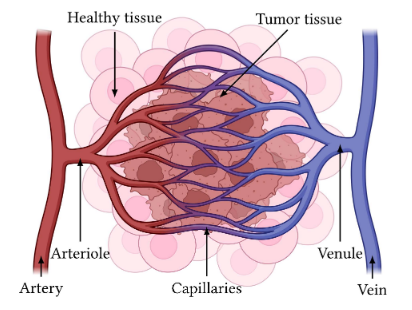
\includegraphics[width=\linewidth]{pictures/schematic_bloodvessels.png}
   \caption{This schematic shows the blood vessels system in healthy and cancerous tissue \cite{Zoofaghari_2023}. This shows the distinct areas used in the system model for the EVs flow modeling.}
   \Description{}
 \end{figure}

\section{Results}
\label{sec: num-results}
Our computational framework used COMSOL Multiphysics to solve the relevant equations with finite element methods. The \textit{Transport of Diluted Species (TDS)} module depicted how EVs move, while the \textit{Single-phase Flow (SPF)} module simulated blood flow. Blood velocity profiles from these flow simulations directly contributed to EV transport calculations, using the parameters listed in \cite{Zoofaghari_2023}. The simulations provided important insights into how EVs interact with tumors and the bloodstream. In tumor regions, we observed a strong buildup of EVs due to the dense tissue structure and lower diffusion rates. This effect resulted in concentration gradients that were 3.5 times higher than those in healthy tissue. This creates significant barriers for capillary access, even when the tissues are close together. 

We assumed uniform EV size in this model to remove the effects of diffusion dispersion and focus only on transport and accumulation dynamics. Since the capillary network has a larger total sectional area than the arteriole and venule, blood flow simulations show that the velocity components in the capillary network are considerably lower and this slow flow helps EV exchange. Only a small percentage of EVs diffuse into capillaries, while most accumulate in tumor areas. After entering the capillaries, EVs are quickly transported into the venule and exit the body, where their concentrations drop rapidly. 

To support effective clearance through circulation, EV transport streamlines ensure that flux is directed toward the vein and increases as it approaches the outlet. The EV penetration rate \( R_s \), calculated over the VCS, shows a clear dependence on tumor size and blood flow parameters. This rate is computed by integrating the EV flux across VCS, accounting for concentration gradients and the component of blood velocity normal to the VCS.

Simulations across different tumor sizes revealed the following key observations regarding $R_s$:
\begin{itemize}
    \item Tumor-derived EVs enter the bloodstream at rates that are inversely proportional to tumor size.

    \item The temporal profiles of EV penetration provide significant diagnostic information:
    \begin{itemize}
        \item Small tumors with 200~\si{\micro\meter} release EVs rapidly, with a peak at approximately 18 hours.
        \item Larger tumors with 600~\si{\micro\meter} produce weaker signals, with peak amplitudes reduced by 60\% and rise times is slowed.
    \end{itemize}
    
    \item Tumor size influences transport resistance, with larger tumors more strongly impeding EV escape.

    \item An increase of 100~\si{\micro\meter} in tumor diameter results in a approximately 30\% reduction in peak EV penetration rate. This relationship enables the detection of tumor size changes for small tumors within the diagnostic time window.
\end{itemize}

\section{Conclusion}
\label{sec: conclusion}
This study presents a comprehensive in silico framework that models the generation, transport, and bloodstream entry of tumor-derived EVs with high spatial and temporal resolution. Through simulations of capillary-tissue dynamics and EV kinetics using COMSOL Multiphysics, we quantified the EV penetration rate $R_s$ as a diagnostic metric, uncovering its strong dependence on tumor size and microenvironmental transport conditions.

Our results demonstrate that even sub-millimeter tumors can generate measurable EV signatures in the bloodstream. Notably, smaller tumors produce sharper and earlier peaks in $R_s$, while larger tumors exhibit delayed and attenuated signals due to increased diffusion resistance and localized EV accumulation. 

The model shows that an increase in tumor diameter of just 100~\si{\micro\meter} can reduce EV penetration rates by over 30\%, highlighting a highly sensitive relationship between tumor size and bloodstream signal strength.

These findings suggest a promising avenue for non-invasive cancer detection using circulating EV profiles, with potential sensitivity down to 50~\si{\micro\meter}. That is well below the threshold of conventional imaging modalities. Furthermore, the temporal evolution of EV release offers a new diagnostic dimension beyond static imaging, enabling early detection and potentially improving patient outcomes.

Future work could aim to extend the model to heterogeneous EV populations, incorporate active cellular uptake mechanisms and validate the computational predictions with in vitro and in vivo data, using a more advanced three-dimensional system model.

\bibliographystyle{ACM-Reference-Format}
\bibliography{my_library}

\end{document}
\endinput